

\documentclass[]{article}
\usepackage[utf8]{inputenc}
\usepackage{amsmath}
\usepackage{graphicx}
\usepackage{csquotes}
\begin{document}


\tableofcontents
\newpage
\section{Einleitung}


Ziel dieser Arbeit ist es, ein Modell zu entwickeln, welches den Zeitpunkt der Laubverfärbung in Nordamerika unter Zuhilfenahme von meteorologischen Variablen möglichst genau vorhersagt. Hierzu werden über einen längeren Zeitraum Klimareanalysedaten mit Satellitenbeobachtungen zur Laubverfärbung verglichen.
\\ \\
Die Laubverfärbung, also das Vertrocknen und Absterben der Blätter in Laubwäldern, ist für Wetter- und Klimamodelle relevant, da sich bei der Verfärbung die Albedo, also der Anteil der nicht zurückgestreuten Strahlung, der Blätter verändert. Außerdem endet die Photosynthese-Aktivität in den Blättern, d. h. die Umwandlung von $CO_2$ in Sauerstoff und die Evaporation nehmen ab, was gerade bei größeren zusammenhängenden Waldstücken einen Einfluss auf Temperatur, $CO_2$-Konzentration und Luftfeuchte in den unteren Schichten hat. Eine einigermaßen zuverlässige Vorhersage des Laubverfärbungszeitpunktes könnte daher Wetter- und Klimamodelle verbessern.
\\ \\
Der genaue Laubverfärbungszeitpunkt ist auch für die Tourismus-Branche relevant, was eine weitere mögliche konkrete Anwendungsmöglichkeit für ein solches Vorhersage-Modell darstellt.
\\ \\
Außerdem soll mit dieser Arbeit am Beispiel der Laubverfärbung untersucht werden, ob und wie aus Klimareanalysedaten mit statistischen Mitteln Erkenntnisse gewonnen werden können, die ansonsten aufwendige Labor- oder Feldversuche erfordern würden.
\\ \\ \\
Für das Modell zur Vorhersage des Laubverfärbungszeitpunktes werden Klimareanalysedaten mit Satellitenbeobachtungen verglichen. An Klimareanalysedaten werden aus der Klimareanalyse ERA-Interim vom ECMWF [Dr. Dick Dee] Variablen wie Temperaturen in verschiedenen Höhen, Luftfeuchte, Druck, Niederschlag und Sonnenscheindauer verwendet. Als Satellitenbeobachtung zur Laubverfärbung wurden zunächst Datensätze zur End-Of-Season-Time des eMODIS-Satelliten Terra verwendet. Diese standen von 2001-2016 mit einer Auflösung von 250m zur Verfügung. Da die Ergebnisse nicht allzu zufriedenstellend waren und die End-Of-Season-Time auch nicht genau den gesuchten Zeitpunkt der Laubverfärbung beschreibt, wurden in einem zweiten Schritt aus NDVI-Daten (Normalized Difference Vegetation Index) des NOAA-AVHRR-Satelliten ein sogenannter "Brownness-Index" und eine "Peak-Brownness-Time" nach [Zhang et al...] berechnet. 
Diese Daten wurden einander räumlich und zeitlich zugeordnet und verglichen, um mit Hilfe von multiplen linearen Regressionen Zusammenhänge zwischen meteorologischen Variablen über die komplette Saison und dem Zeitpunkt der Laubverfärbung herzustellen. Daraus soll schließlich ein Modell entstehen, welches den Zeitpunkt der Laubverfärbung schon möglichst früh und möglichst genau vorhersagen kann. Da der Zeitpunkt der Laubverfärbung sehr stark von der Art des jeweiligen Baumes bzw. Waldstückes abhängt, wird in dieser Arbeit mit daten von Nordamerika gearbeitet, wo es sehr große zusammenhängende homogene Waldgebiete gibt. Außerdem wird mit einer relativ hohen räumlichen Auflösung gearbeitet. Gemischte Waldgebiete werden zu einer Mischform mit einem mittleren Laubverfärbungszeitpunkt zusammengefasst [-> Zhang et. al]. Es werden für jeden Pixel Zeitreihen analysiert. Ein Vergleich mit anderen Pixeln geschieht nicht, da nicht davon ausgegangen werden kann, dass die Bedingungen vergleichbar sind. Auch zeitlich sind die Daten nur dann vergleichbar, wenn sich Zusammensetzung und Zustand des Waldstücks unter einem Pixel über den Beobachtungszeitraum nicht wesentlich verändern, wovon hier ausgegangen wird.

\newpage
\section{Meteorologische Grundlagen}
\subsection{Klimareanalysen}
Ein großer Teil der Daten, die in dieser Arbeit verwendet werden, stammt aus der Klimareanalyse Era-Interim vom Europäischen Zentrum für Mittelfrist-Wettervorhersagen (ECMWF). Klimareanalysen sind ein systematischer Ansatz, Datensätze für Klima-Monitoring und Forschungszwecke zu gewinnen. Sie sind eine vierdimensionale Beschreibung des Zustands der Atmosphäre, bestehend aus einem numerischen Wettervorhersagemodell und einem Datenassimilationssystem. Das Modell gibt für jeden Zeitschritt eine dynamisch konsistente Schätzung des Zustands der Atmosphäre aus. Über ein statisches Datenassimilationssystem wird es laufend an Beobachtungsdaten angeglichen. Diese Beobachtungsdaten stammen von Wetterstationen, Radionsonden, Satelliten, Bojen, Flugzeug- und Schiffsmeldungen. Sie stellen die einzige Veränderliche Komponente einer Reanalyse dar, da Anzahl und Qualität der Beobachtungsdaten durchaus schwanken können. 

Klimareanalysen liefern Datensätze mit hunderten von Variablen aus einem konsistenten System bei konstanter räumlicher und zeitlicher Auflösung über mehrere Dekaden. Modellauflösung und Fehler werden dabei bei neuen Reanalysen ständig verbessert. Über die Datenassimilationssysteme werden teilweise Millionen von Beobachtungen aufgenommen, was von Hand wohl kaum möglich wäre. Die Einheitlichen konsistenten Datensätze vereinfachen die Arbeit für viele Anwendungen. Die Beobachtungen allerdings, und damit die Verlässlichkeit einer Reanalyse, können abhängig von Ort, Zeit und Variable stark schwanken. Der wechselhafte Beobachtungsmix kann zu falschen Trends und Variabilitäten im Output einer Reanalyse führen. Außerdem musste festgestellt werden, dass diagnostische Variablen im Zusammenhang mit dem hydrologischen Kreislauf, wie z. B. Niederschlag und Evaporation, mit Vorsicht verwendet werden sollten.

[https://climatedataguide.ucar.edu/climate-data/atmospheric-reanalysis-overview-comparison-tables zitieren]
\subsection{NDVI}
Der \textit{Normalized Divergence Vegetation Index} (NDVI) ist ein Index, der aus Satellitenbeobachtungen einen Wert für die Vegetationsdichte in einem Pixel ausgibt. Hierzu werden zwei Kanäle miteinander verglichen: Sichtbares Licht ($0,4-0,7 \mu m$ Wellenlänge) und Licht aus dem Nah-Infrarotbereich ($0,7 - 1,1 \mu m$ Wellenlänge). Chlorophyll, der Stoff der in Pflanzen für die Photosynthese sorgt, absorbiert sichtbares Licht verhältnismäßig stark. Die Zellstruktur der Blätter dagegen reflektiert Licht aus dem Nah-Infrarotbereich sehr stark. Diese beiden Effekte werden werden für den NDVI verwendet, welcher sich aus folgender Formel berechnen lässt:
\begin{equation}
NDVI=\frac{NIR - VIS}{NIR + VIS}
\end{equation}
$NIR$ steht hier für Reflexion im Nah-Infrarotbereich, $VIS$ für Reflexion im sichtbaren Wellenlängenbereich, beide Werte in $\%$.
\begin{figure}
	\centering
  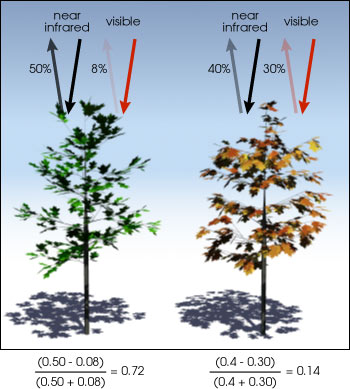
\includegraphics[width=0.75\textwidth]{ndvi_example.jpg}
	\caption{Beispielhafte NDVI-Werte}
	\label{fig1}
\end{figure}
Abbildung \ref{fig1} zeigt die NDVI-Berechnung an zwei beispielhaften Fällen: Links die Strahlungssituation über verhältnismäßig dichter Vegetation mit aktiver Photosynthese und rechts einen Fall von eher schwacher, trockener oder inaktiver Vegetation. Im linken Fall wird verhältnismäßig wenig sichtbares Licht reflektiert, gleichzeitig ist die Reflexion von Nah-Infrarot-Licht verhältnismäßig hoch. Dies führt zu einem relativ hohen NDVI. Im rechten Fall wird deutlich mehr sichtbares Licht reflektiert, dabei ist die Reflexion von Nah-Infrarot-Licht schwächer, was zu einem niedrigen NDVI führt.

Der NDVI kann Werte zwischen -1 und 1 erreichen, wobei negative Werte eher selten sind. Ein hoher NDVI steht für dichte Vegetation mit hoher Photosyntheseaktivität, ein niedriger NDVI steht dagegen für wenig Vegetation bzw. wenig Photosyntheseaktivität in einem Pixel.

[https://earthobservatory.nasa.gov/Features/MeasuringVegetation/measuring\_vegetation\_2.php]
\subsection{Statistik?}
\section{verwendete Daten}
\subsection{Era-Interim}
Für diese Arbeit wurden die Daten der Reanalyse Era-Interim verwendet. Die Entscheidung für Era-Interim fiel, da diese Reanalyse sich bereits in vielen Untersuchungen als zuverlässige Datenquelle bewiesen hat. Der verfübgare Zeitraum deckt gut den Zeitraum der verwendeten Satellitendaten ab. Außerdem war der Zugang zu diesen Daten relativ einfach, was in der begrenzten Zeit, die für eine Bachelorarbeit zur Verfügung steht, durchaus auch eine Rolle spielt. Mit einer Auflösung von etwa 80 km sind die Era-Interim-Daten deutlich gröber aufgelöst als die verwendeten Satellitendaten ($250m$ bzw $0,05^{\circ}$). Eine mit den Satellitendaten vergleichbar hoch aufgelöste Reanalyse gibt es allerdings nicht für den gesuchten Zeitraum und die gesuchte räumliche Ausdehnung.

Die Reanalyse Era-Interim stellt Daten von 1979 bis 2018 zur Vefügung, mit einer Verzögerung von etwa zwei Monaten zur Qualitätssicherung wird sie kontinuierlich mit aktuellen Beobachtungsdaten verlängert.  
\\
\\

\subsection{MODIS-EOST}
Für die Beobachtung der Laubverfärbung werden in dieser Arbeit zwei verschiedene Datensätze herangezogen. Zum einen ein Datensatz zur \textit{End Of Season Time}, bereitgestellt vom U. S. Geological Survey (USGS). Dieser Datensatz wurde produziert aus NDVI-Beobachtungen der \textit{MODerate-resolution Imaging Spectroradiometer(MODIS)}-Sensoren der NASA-Satelliten Terra und Aqua. Diese Satelliten überfliegen die Erde alle ein bis zwei Tage. Alle sieben Tage ist ein korrigierter NDVI-Wert mit einer Auflösung von $250m \cdot 250m$ verfügbar.

Die \textit{End Of Season Time} identifiziert den Tag, an dem die Photosyntheseaktivität der Vegetationsoberfläche das Ende der Seneszenz erreicht. Hierzu werden für jeden Pixel geglättete NDVI-Beobachtungs-Zeitreihen erstellt. Dann wird der Reihe nach jeder Wert mit einem vorwärts gerichteten \textit{moving-average} verglichen. Der Tag, an dem der NDVI der geglätteten Zeitreihe unter den vorwärts gerichteten \textit{moving average}-Wert fällt, wird als \textit{End Of Season Time} definiert. Um eine Genauigkeit von einem Tag zu erreichen, wird zwischen den korrigierten NDVI-Werten linear interpoliert. Die Länge des \textit{moving-average}-Fensters wird auf 36 Wochen festgelegt. Verfügbar ist die MODIS-\textit{End Of Season Time} für die Jahre 2001-2016. Der Datensatz deckt räumlich die östliche Hälfte der USA ab.

Die \textit{End of Season Time} bezeichnet daher nicht direkt den Zeitpunkt der Laubverfärbung, sondern vielmehr das absolute Ende der Phase der Photosyntheseaktivität. Dieser Datensatz lässt jedoch Rückschlüsse auf die zu untersuchende Vegetations-Phänologie zu, es wird angenommen, dass bei einer verhältnismäßig frühen Laubverfärbung auch die \textit{End Of Season Time} früher eintritt und umgekehrt. Außerdem kann es hilfreich sein, die \textit{End Of Season Time} mit anderen Datensätzen zur Laubverfärbung zu vergleichen.
\subsection{NOAA AVHRR NDVI}
Der zweite verwendete Datensatz von Satellitenbeobachtungen zur Laubverfärbung ist ein NDVI-Datensatz des AVHRR(Advanced Very High Resolution Radiometer)-Sensors von polarumlaufenden NOAA (National Oceanic and Atmospheric Administration)-Satelliten. Dieser Datensatz stellt von 1982 bis heute täglich global NDVI-Werte mit einer Auflösung von $0,05^\circ$ zur Verfügung. Da der NDVI bei Bewölkung nicht korrekt gemessen werden kann, sind die nicht nachbearbeiteten täglichen NDVI-Werte häufig fehlerhaft. Der Datensatz liefert hierzu sogenannte \enquote{Quality Assurance}-Flags mit, die für jeden Pixel unter anderem Einflüsse von Wolken, Wolkenschatten und Wasseroberflächen angeben. Mit Hilfe dieser QA-Flags können potentiell fehlerhafte Werte direkt ausgeschlossen werden. Aus diesem NDVI-Datensatz wird dann ein \enquote{Temporally Normalized Brownness Index} nach [Zhang et al] berechnet.       
\section{Datenverarbeitung/Preprocessing}
\subsection{Era-Interim}
Aus den bei Era-Interim verfügbaren Variablen wurden acht ausgewählt, die in dieser Arbeit mit Satellitendaten verglichen werden. Zwei weitere Variablen wurden aus diesen Daten berechnet. Dies sind zum einen die relative Feuchte und zum anderen die Wachstumsgradtage. Die relative Feuchte wurde aus 2m-Temperatur und 2m-Taupunkttemperatur mithilfe folgender Formeln berechnet (mit $T=$ 2m-Temperatur in $^{\circ} C$ und $TD=$ 2m-Taupunkttemperatur in $^{\circ}C$):

\begin{equation}
relhum=\frac{e_{sat}(TD)}{e_{sat}(T)}
\end{equation}
Der Sättigungsdampfdruck $e_{sat}$ abhängig von der Temperatur $T$ wird über die Magnusformel berechnet [nach Sommer, D. 1990 ...] :
\begin{equation}
e_{sat}(T)=6,112hPa\cdot\exp\left(\frac{17,62 \cdot T}{243,12 ^{\circ}C + T}\right)
\end{equation}
Dann ergibt sich:
\begin{equation}
relhum(T,TD)=\exp\left(17,62\cdot\left(\frac{TD}{TD+243,12^{\circ}C}-\frac{T}{T+243,12^{\circ}C}\right)\right)
\end{equation}
Wachstumsgradtage bezeichnen eine Größe, die relativ häufig im Zusammenhang mit dem Wachstum von Pflanzen verwendet wird. Mit Wachstumsgradtagen wird die Anzahl Tage bezeichnet, an denen die Durchschnittstemperatur über einem
Schwellwert liegt, gewichtet mit der Differenz zum Schwellwert. Es gibt unterschiedliche Methoden, diese Wachstumsgradtage zu berechnen. In dieser Arbeit wird die folgende Formel berechnet:
\begin{equation}
WGT=\begin{cases}
T_{mean}-T_0 & \;\;\;\text{ wenn }  T_{mean}>T_0 \\
0 & \; \;\;\text{ sonst} 
\end{cases}
\end{equation}
Hierbei bezeichnet $T_{mean}$ die mittlere 2m-Temperatur eines Tages und $T_0$ die Schwellwerttemperatur. Für diese Arbeit wurde die Schwellwerttemperatur auf $T_0=10^\circ C$ gesetzt. \\

\begin{tabular}{|c|c|}
	\multicolumn{2}{c}{verwendete Variablen}\\
	\hline
	Schneehöhe& Era-Interim\\
	\hline
	Schneefall& Era-Interim\\
	\hline
	2m-Temperatur& Era-Interim \\
	\hline
	2m-Taupunkttemperatur& Era-Interim\\
	\hline
	Bodentemperatur&Era-Interim\\
	\hline
	Evaporation& Era-Interim\\
	\hline
	Sonnenscheindauer& Era-Interim\\
	\hline
	Niederschlag& Era-Interim\\
	\hline
	Wachstumsgradtage& berechnet\\
	\hline
	relative Feuchte& berechnet\\
	\hline
\end{tabular}

\subsection{TNBI}
\subsection{Gitterpunkte räumlich zuordnen?}
\section{Ergebnisse}

\end{document}